\documentclass[11pt]{article}
\usepackage[margin=2.5cm]{geometry}
\usepackage{amsmath,amssymb,booktabs,graphicx}
\usepackage[hidelinks]{hyperref}
\newcommand{\N}{\mathcal{N}}
\title{A parts world where the cat--dog product is exact}
\author{Worked example for claim 9 of the overlap-dial idea map}
\date{}
\begin{document}
\maketitle

\section*{What this example shows}

A two-dimensional toy can only show a chimera as a midpoint, because each slot holds one number.
Real cat--dog chimeras are mostly mosaics, where some parts come from the cat and others from the dog.
This example uses images of $D = 16$ pixels, drawn as $4 \times 4$ tiles, and experts that are Gaussians
or mixtures of Gaussians. Every product below is then exact in closed form, with no grid and no sampler.
It produces three outcomes from the same two concepts: a mosaic, a midpoint blend, and two animals side
by side. Which one appears depends only on where each expert is consistent, which is a property of its
training data.

\begin{figure}[h]
\centering
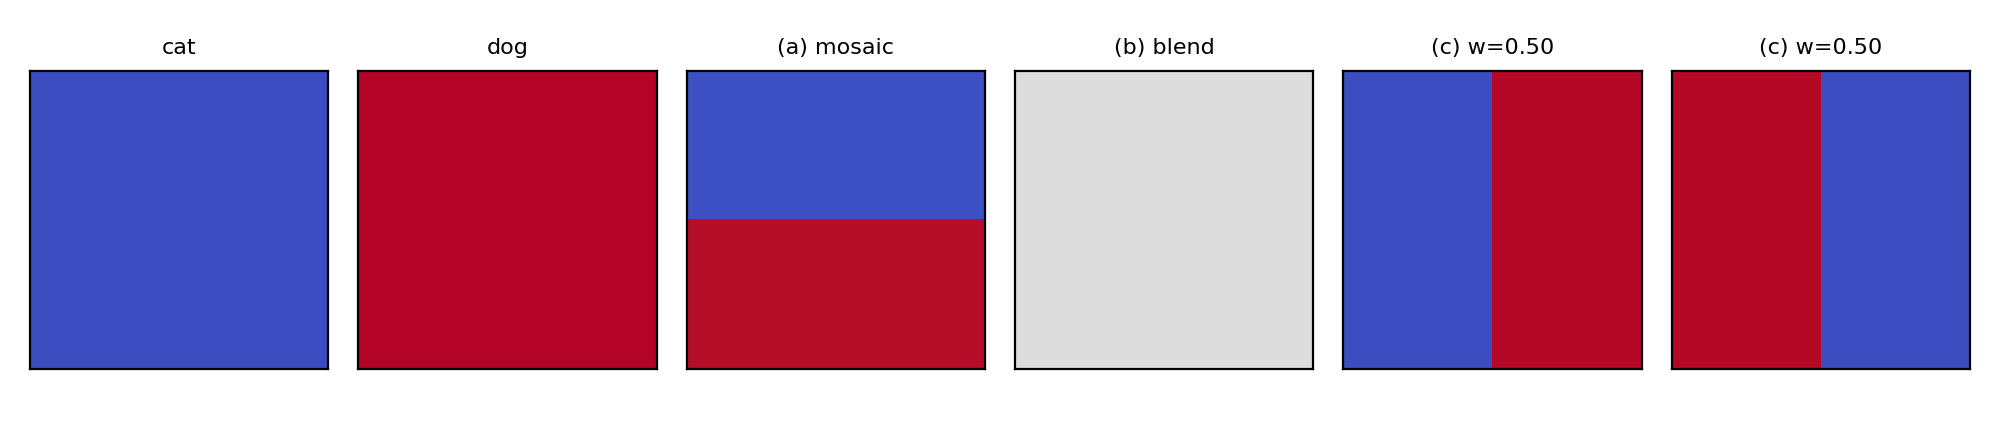
\includegraphics[width=\textwidth]{parts-world-tiles.png}
\caption{Each tile is one image: blue is the cat value $+1$, red is the dog value $-1$, grey is $0$.
The cat and dog tiles are the experts' means. The other tiles are the means of the exact product in
settings (a), (b) and (c) below, and $w$ is a product component's weight.}
\end{figure}

\section*{The one identity everything uses}

For two Gaussians with diagonal covariances,
\begin{equation}
\N(x;\mu_a,\Sigma_a)\,\N(x;\mu_b,\Sigma_b) \;=\; Z\,\N(x;\mu,\Sigma),
\end{equation}
\begin{equation}
\Sigma = \left(\Sigma_a^{-1} + \Sigma_b^{-1}\right)^{-1}, \qquad
\mu = \Sigma\left(\Sigma_a^{-1}\mu_a + \Sigma_b^{-1}\mu_b\right), \qquad
Z = \N(\mu_a;\,\mu_b,\,\Sigma_a + \Sigma_b).
\end{equation}
The precisions add, and the mean is the precision-weighted mean, pixel by pixel. $Z$ is how much the two
experts overlap: when it is tiny, the product exists mathematically but sits where neither expert would
ever put a sample.

For mixtures $p_A = \sum_i \pi_i \N(\mu_i,\Sigma_i)$ and $p_B = \sum_j \rho_j \N(\nu_j,\Lambda_j)$,
the product is a mixture over every pair of components,
\begin{equation}
p_A\,p_B \;\propto\; \sum_{i,j} w_{ij}\,\N(x;\mu_{ij},\Sigma_{ij}), \qquad
w_{ij} \propto \pi_i\,\rho_j\,\N(\mu_i;\,\nu_j,\,\Sigma_i + \Lambda_j),
\end{equation}
with $\mu_{ij},\Sigma_{ij}$ from (2). The weights are exact too.

\section*{Setting (a): complementary consistency gives a mosaic}

The cat expert has mean $+1$ on every pixel, with variance $0.01$ on the head (the top 8 pixels) and $1$
on the body (the bottom 8). Its training cats have consistent heads and varied bodies. The dog expert has
mean $-1$, variance $1$ on the head and $0.01$ on the body. Per head pixel,
\[
\mu_{\text{head}} = \frac{100\cdot(+1) + 1\cdot(-1)}{100 + 1} = +0.980,
\qquad
\mu_{\text{body}} = \frac{1\cdot(+1) + 100\cdot(-1)}{1 + 100} = -0.980.
\]
The product's mean is a cat head on a dog body. On each pixel the more consistent expert wins.
Here $\log Z = -46.5$.

\section*{Setting (b): both consistent everywhere gives a blend}

Both experts have variance $0.01$ on every pixel. Then
\[
\mu = \frac{100\cdot(+1) + 100\cdot(-1)}{200} = 0, \qquad \sigma = \sqrt{0.005} = 0.071 .
\]
Every pixel is grey: neither cat nor dog. That mean is $10$ standard deviations from each expert's mean on
every pixel, and $\log Z = -1583.4$. The product is well defined, yet neither expert would ever produce a
sample near it. This is the midpoint chimera of the two-dimensional slot toy, and the empty intersection of
the ring-times-bar toy, seen in sixteen dimensions.

\section*{Setting (c): position variation gives two animals}

Each expert is a mixture of two placements with weight $0.5$ each: the animal fills the left half (the left
two columns, variance $0.01$) and the other half is loose (mean $0$, variance $1$), or the mirror image.
The product has four component pairs, with weights from (3):

\begin{center}
\begin{tabular}{lrr}
\toprule
pair & $\log w_{ij}$ (unnormalised) & normalised weight \\
\midrule
cat left $\times$ dog left   & $-803.2$ & $0.00$ \\
cat left $\times$ dog right  & $-24.1$  & $0.50$ \\
cat right $\times$ dog left  & $-24.1$  & $0.50$ \\
cat right $\times$ dog right & $-803.2$ & $0.00$ \\
\bottomrule
\end{tabular}
\end{center}

The pairs that put both animals in the same half carry $e^{-779}$ of the weight of the pairs that put them
side by side. The product is two animals, one per half, in either arrangement. This is co-occurrence,
obtained from the same product operator as (b), because the training data showed each animal in more than
one place.

\section*{What reverse diffusion does to setting (a)}

Under the variance-preserving forward process, a Gaussian expert $\N(\mu,\Sigma)$ becomes
$\N(\sqrt{\bar\alpha}\,\mu,\ \bar\alpha\Sigma + (1-\bar\alpha)I)$ at noise level $\bar\alpha$. At
$\bar\alpha = 0.5$, the head variances become $0.5\cdot 0.01 + 0.5 = 0.505$ for the cat and
$0.5\cdot 1 + 0.5 = 1.0$ for the dog. The cat's precision advantage shrinks from $100{:}1$ to about
$2{:}1$. The product of the noised experts, which is what summed scores target, puts the head at
\[
\frac{1.98\cdot 0.707 + 1.0\cdot(-0.707)}{2.98} = 0.233,
\]
while the noised product, the correct intermediate target, puts it at $\sqrt{0.5}\cdot 0.980 = 0.693$.
The gap is the error Du et al.\ (2023, p.~4, eqs.~11--12) describe, computed exactly here. Annealed MCMC
targets each noise level's product directly and does not follow this path.

\section*{Where the numbers come from}

\texttt{parts\_world.py} in this folder computes every number above and writes them to
\texttt{numbers.json}. It draws the figure as well.

\end{document}
